\documentclass{scrartcl}
\usepackage{color}
\usepackage{url}
\usepackage{cite}
\usepackage{eucal}
\usepackage{fancybox}
\usepackage{amsmath}
\usepackage{epsfig}
\usepackage{amssymb}
\usepackage{amsfonts}
\usepackage{hyperref}
\usepackage{listings}
\usepackage{caption,subcaption}
%
\newcommand{\TODO}[1]{\textcolor{red}{\boxed{\mathbf{TODO }} {\textit{#1}} }}
\newcommand{\REMARK}[1]{\textcolor{blue}{\boxed{\mathbf{Remark }} {\textit{#1}} }}
\newcommand{\todo}{\TODO}
\newcommand{\remark}{\REMARK}
\newcommand{\email}[1]{\texttt{#1}}
%
\begin{document}

\title{RNav - R-Tree Navigation Helper on Google App Engine}
\subtitle{CS 764 - Spring 2013 - Innovation Project}

\author{
Aaron Gorenstein\\
	\email{agorenst@cs.wisc.edu}
\and
Rebecca Lam\\
	\email{rjlam@cs.wisc.edu}
\and
Cathrin Weiss\\
	\email{cweiss@cs.wisc.edu}       
}

\date{\today}

\maketitle

%====== OVERVIEW =======================
\section{Overview}
\label{sec:intro}
Google's App Engine allows for rapid development of web applications without worrying about maintenance or scalability\footnote{\url{https://developers.google.com/appengine/}}. It follows the key-value storage paradigm for persistent as well as in-memory storage.

We developed a route planning application leveraging an R-Tree structure on the server side. Using the California Roads data set~\cite{Online:cardata}, we provide route guidance functionality given two input points A and B (assuming A and B are within the described area). The project consists of six components:
\begin{enumerate}
\item The R-Tree data loader, which will convert the geo data into a key-value-compatible R-Tree index (this and part 1 may possibly be combined)
\item The actual R-Tree index, which can process the native R-Tree operations,
\item An algorithm module to compute the shortest route from point A to point B,
\item A simple query engine to process navigation requests, 
\item A query frontend for entering route requests, and
\item A result generator to present the final route to the user. 
\end{enumerate}
One of the challenges was the mapping of the traditional R-Tree implementation in~\cite{DBLP:conf/sigmod/Guttman84} to Google's key-value store. 

The architecture of our project is presented in section~\ref{sec:architecture}. 

%====== ARCHITECTURE ==================
\section{Architecture}
\label{sec:architecture}
\begin{figure}[h]
\begin{center}
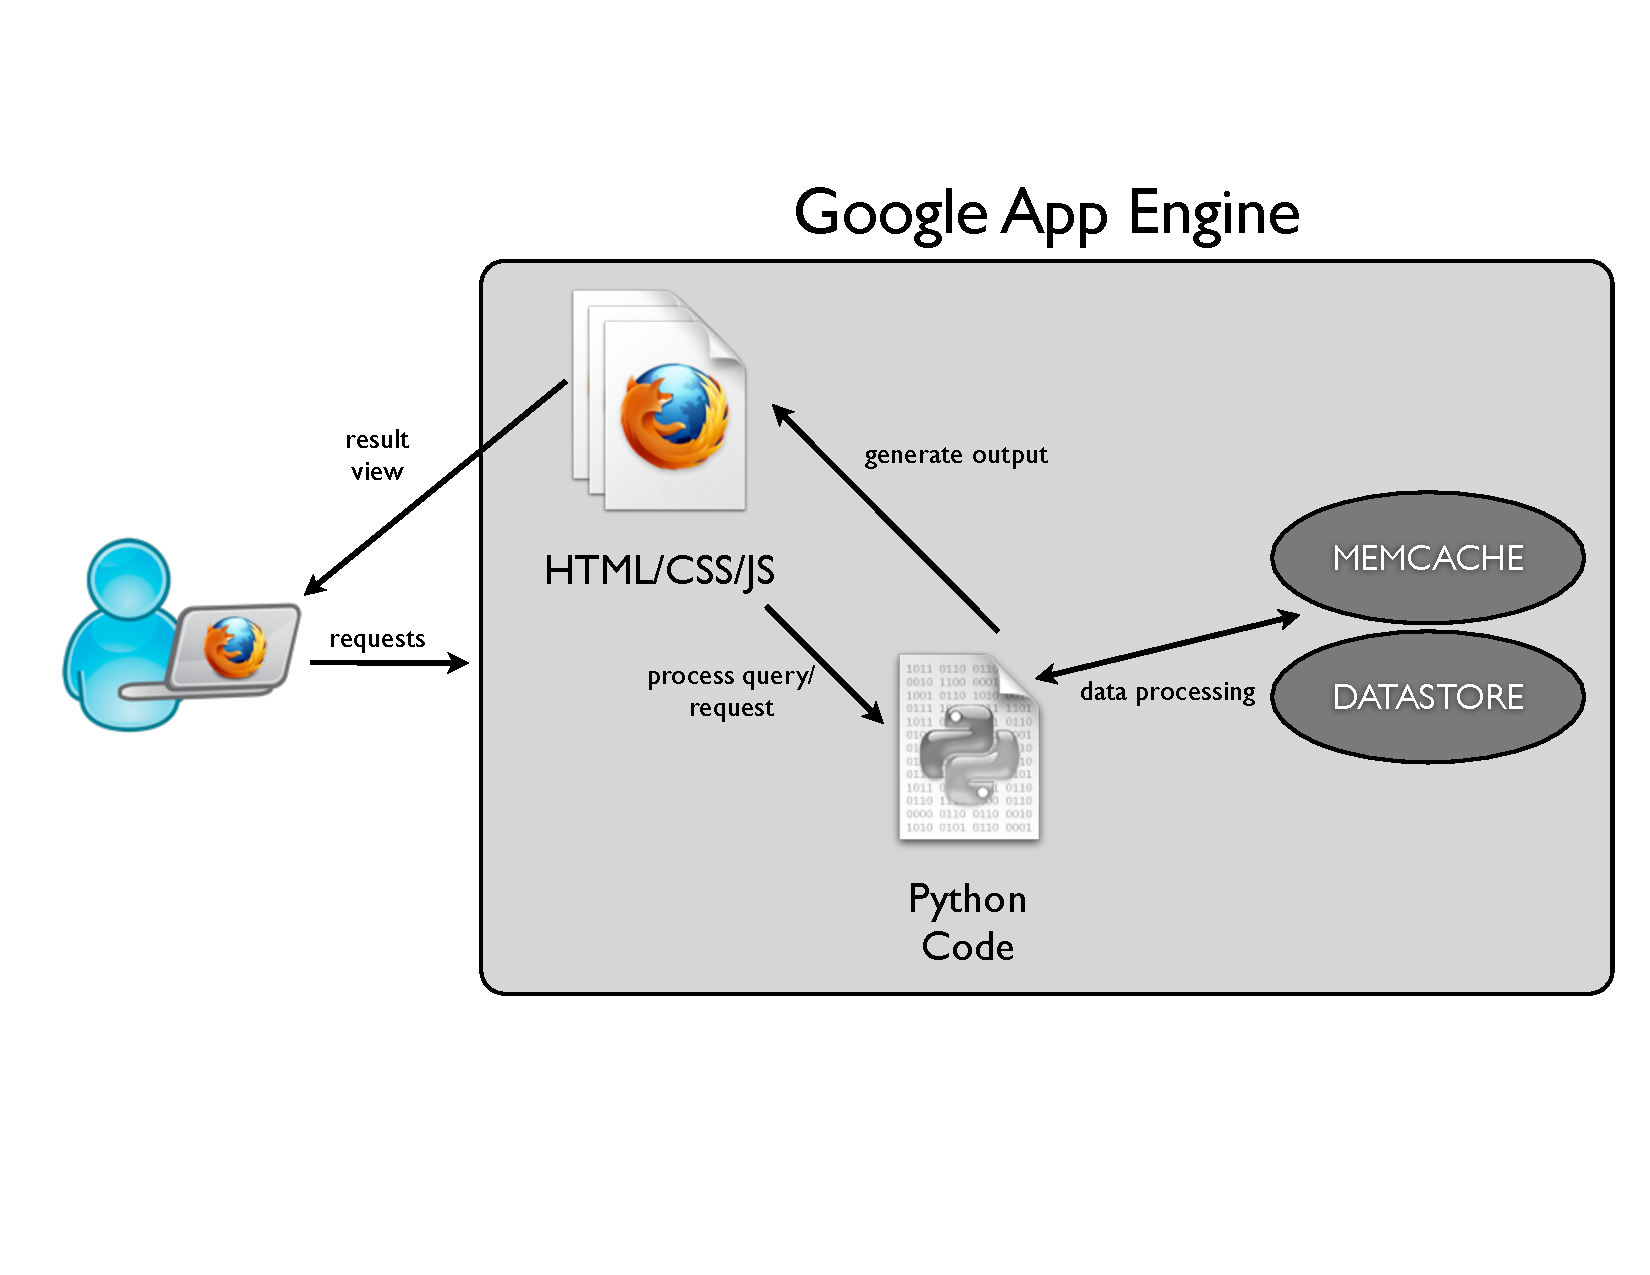
\includegraphics[scale=0.3]{fig/gapps1}
\caption{Google App Engine default architecture}
\label{fig:gappsArch}
\end{center}
\end{figure}

\begin{figure}[h]
\begin{center}
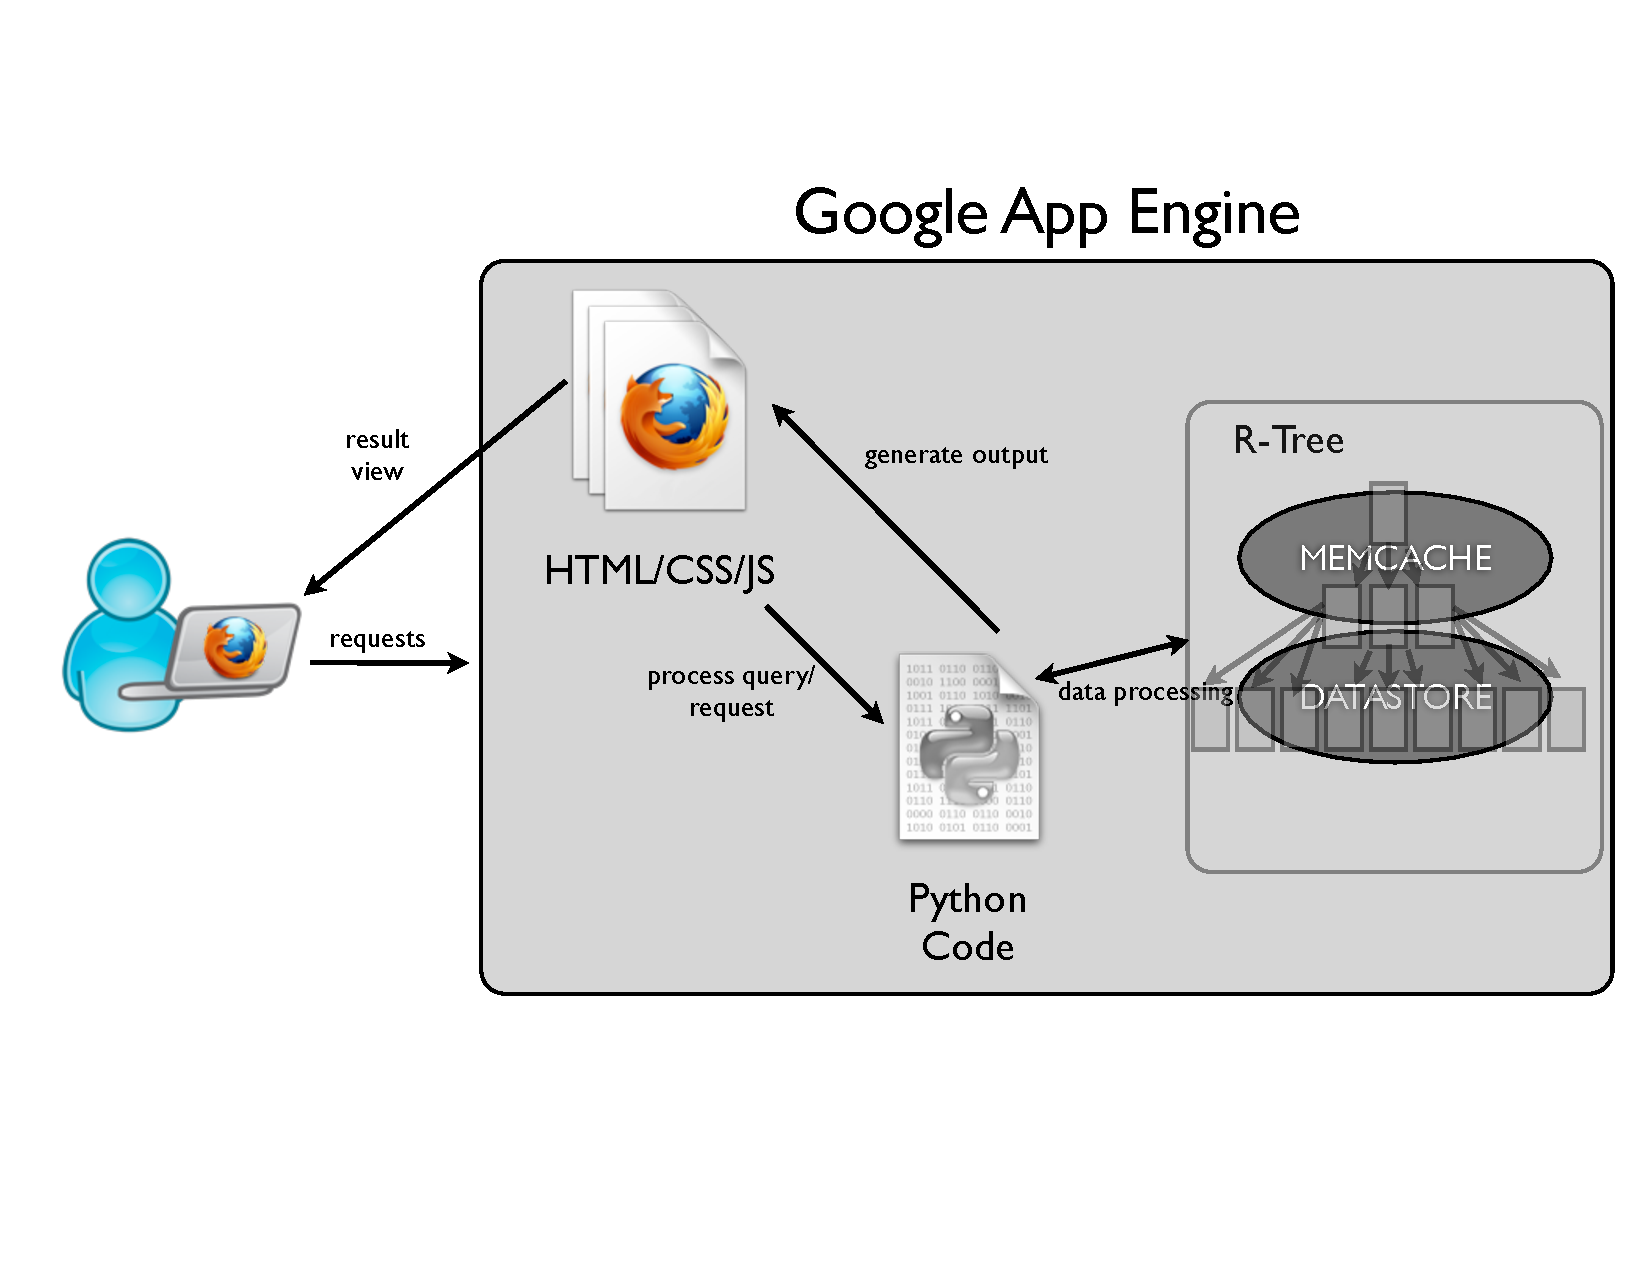
\includegraphics[scale=0.3]{fig/gapps2}
\caption{Google App Engine architecture with R-Tree index}
\label{fig:gappsArch2}
\end{center}
\end{figure}

The architecture of a common Google App Engine application is depicted in figure~\ref{fig:gappsArch}. A user makes a web request, which gets forwarded to the Python backend, which itself processes the request and interacts with the data store. The data can either be stored persistently or in memory. The latter is referred to as ``Memcache''. Usually data access follows standard key-value protocols. For our project we created an R-Tree index within the key-value data store in order to speed up spatial requests. This is schematically shown in figure~\ref{fig:gappsArch2}. The actual R-Tree layout and implementation is described in section~\ref{sec:implementation}.

Additionally, we implemented a route-finding algorithm, which takes as input the list of roads retrieved via the R-Tree lookup and generates a route from point A to point B. The resulting is presented to the querying user in a graphical result view.

%====== IMPLEMENTATION ==================
\section{Implementation}
\label{sec:implementation}
\subsection{R-Tree layout in Google's key-value store}
\TODO{fill in text}

\subsection{Navigation Algorithm}
\TODO{fill in text}
\bibliographystyle{abbrv}
\bibliography{main}

\end{document}
